\section{Proposed Methods}
In this section, we introduce the use of AC as a concrete speech processing system. We first define a binary neural interface that transforms continuous acoustic features into sparse, spike-like representations compatible with AC areas, thereby bridging the gap between real-valued speech signals and the discrete assembly dynamics assumed by AC. We then specify the architectural organisation and connectivity of these areas to support two core functions: temporal segmentation and segment classification. For temporal segmentation, we configure a fixed-dynamics hierarchy of refractory assembly areas that expose phone- and word-level boundaries in continuous speech. For segment classification, we introduce plastic, per-class recurrent areas whose learned activation trajectories encode phone and word identities. Taken together, these components form a fully specified AC-based speech processing architecture that can be instantiated on real speech corpora and evaluated on standard boundary detection and classification tasks.
Figure~\ref{fig:conceptual_overview} provides a conceptual overview of the framework, highlighting the three novel contributions and where they sit in the processing pipeline.
\begin{figure}[t]
\centering
\tikzset{
  encode/.style={draw, rounded corners=2pt, minimum height=0.45cm, minimum width=1.0cm,
               font=\tiny, inner sep=2pt, align=center, fill=orange!18, thick},
  area/.style={draw, rounded corners=2pt, minimum height=0.45cm, minimum width=1.0cm,
               font=\tiny, inner sep=2pt, align=center, fill=blue!15, thick},
  readout/.style={draw, rounded corners=2pt, minimum height=0.45cm, minimum width=0.9cm,
               font=\tiny, inner sep=2pt, align=center, fill=red!12, thick},
  task/.style={draw, rounded corners=2pt, minimum height=0.45cm, minimum width=0.9cm,
               font=\tiny, inner sep=2pt, align=center, fill=green!15},
  arr/.style={-{Stealth[length=2.5pt]}, semithick},
  clabel/.style={font=\tiny\bfseries, text=black!70},
}

\begin{tikzpicture}[x=0.85cm, y=1cm]

\begin{scope}[shift={(0,0)}]
  \draw[thick, rounded corners=2pt] (-0.55,-0.35) rectangle (0.55,0.35);
  \draw[gray!70, semithick] plot[domain=-0.4:0.4, samples=40, smooth]
    (\x, {0.2*sin(1800*\x)*exp(-4*\x*\x)});
  \node[font=\tiny, below] at (0, -0.38) {Speech};
\end{scope}

\coordinate (fork) at (0.75, 0);
\draw[arr] (0.55, 0) -- (fork);

\node[encode] (mel) at (2.2, 0.85) {Prob.\ mel\\[-1pt]binarisation};
\node[area] (refr) at (3.9, 0.85) {Refractory\\[-1pt]hierarchy};
\node[readout] (change) at (5.5, 0.85) {$c^{(t)}$};
\node[task] (bd) at (6.8, 0.85) {Boundary\\[-1pt]detection};

\draw[arr] (fork) |- (mel);
\draw[arr] (mel) -- (refr);
\draw[arr] (refr) -- (change);
\draw[arr] (change) -- (bd);

\node[encode] (mfcc) at (2.2, -0.85) {Pop-coded\\[-1pt]MFCCs};
\node[area] (perclass) at (3.9, -0.85) {Per-class\\[-1pt]Recurrent};
\node[readout] (res) at (5.5, -0.85) {$R_c$};
\node[task] (cl) at (6.8, -0.85) {Segment\\[-1pt]classif.};

\draw[arr] (fork) |- (mfcc);
\draw[arr] (mfcc) -- (perclass);
\draw[arr] (perclass) -- (res);
\draw[arr] (res) -- (cl);

\node[clabel] at (2.2, 1.7) {(i) Encoding};
\node[clabel] at (3.9, 1.7) {(ii) Architecture};
\node[clabel] at (5.5, 1.7) {(iii) Read-out};

\draw[densely dashed, gray!40] (1.2, 1.5) -- (1.2, -1.4);
\draw[densely dashed, gray!40] (3.05, 1.5) -- (3.05, -1.4);
\draw[densely dashed, gray!40] (4.75, 1.5) -- (4.75, -1.4);
\draw[densely dashed, gray!40] (6.1, 1.5) -- (6.1, -1.4);

\node[font=\tiny\itshape, text=black!45] at (5.5, 1.2) {$\beta{=}0$};
\node[font=\tiny\itshape, text=black!45] at (5.5, -1.2) {$\beta{>}0$};

\end{tikzpicture}

\caption{Conceptual overview. Speech is processed by two separate AC pipelines. \textbf{Top:} binarised mel frames drive a frozen-weight refractory hierarchy; the change signal $c^{(t)}$ marks boundaries ($\beta{=}0$). \textbf{Bottom:} population-coded MFCCs drive per-class RecurrentAreas; resonance scoring $R_c$ identifies the class ($\beta{>}0$). Columns mark the three contributions: (i)~neural encoding, (ii)~area architecture, (iii)~task read-out.}
\vspace{-10pt}
\label{fig:conceptual_overview}
\end{figure}


\subsection{Binary Neural Encoding for Speech}

AC areas operate on sparse binary vectors~\cite{papadimitriouBrainComputationAssemblies2020}. We therefore require an encoding that converts continuous speech features to ``binary spike trains'' while preserving relevant acoustic structure. To this end, we employ two complementary encodings that emphasise different properties of the signal.

\subsubsection{Probabilistic Mel Encoding}
\label{sec:prob_bin}

To preserve fine-grained temporal variation for tasks that require precise boundary recognition, mel-spectral frames are converted into binary vectors through probabilistic sampling, as shown in Figure~\ref{fig:prob_bin}. Given a mel feature vector $\mathbf{x}$, each component $x_i$ is first optionally compressed using a power-law transformation
\begin{equation}
p_i = x_i^{\gamma}, \gamma \le 1
\end{equation}
which reduces dynamic range when $\gamma \le 1$. Each $p_i$ is then interpreted as the firing probability of an input neuron, and a Bernoulli sample is drawn independently for each dimension. As a result, higher-energy mel bins are more likely to activate input neurons, producing sparse stochastic spike patterns that reflect local spectral energy. This encoding preserves frame-to-frame variability in the mel spectrogram and supports dynamic state transitions in downstream AC areas (Figure~\ref{fig:prob_bin}).

\begin{figure}[t]
    \centering
    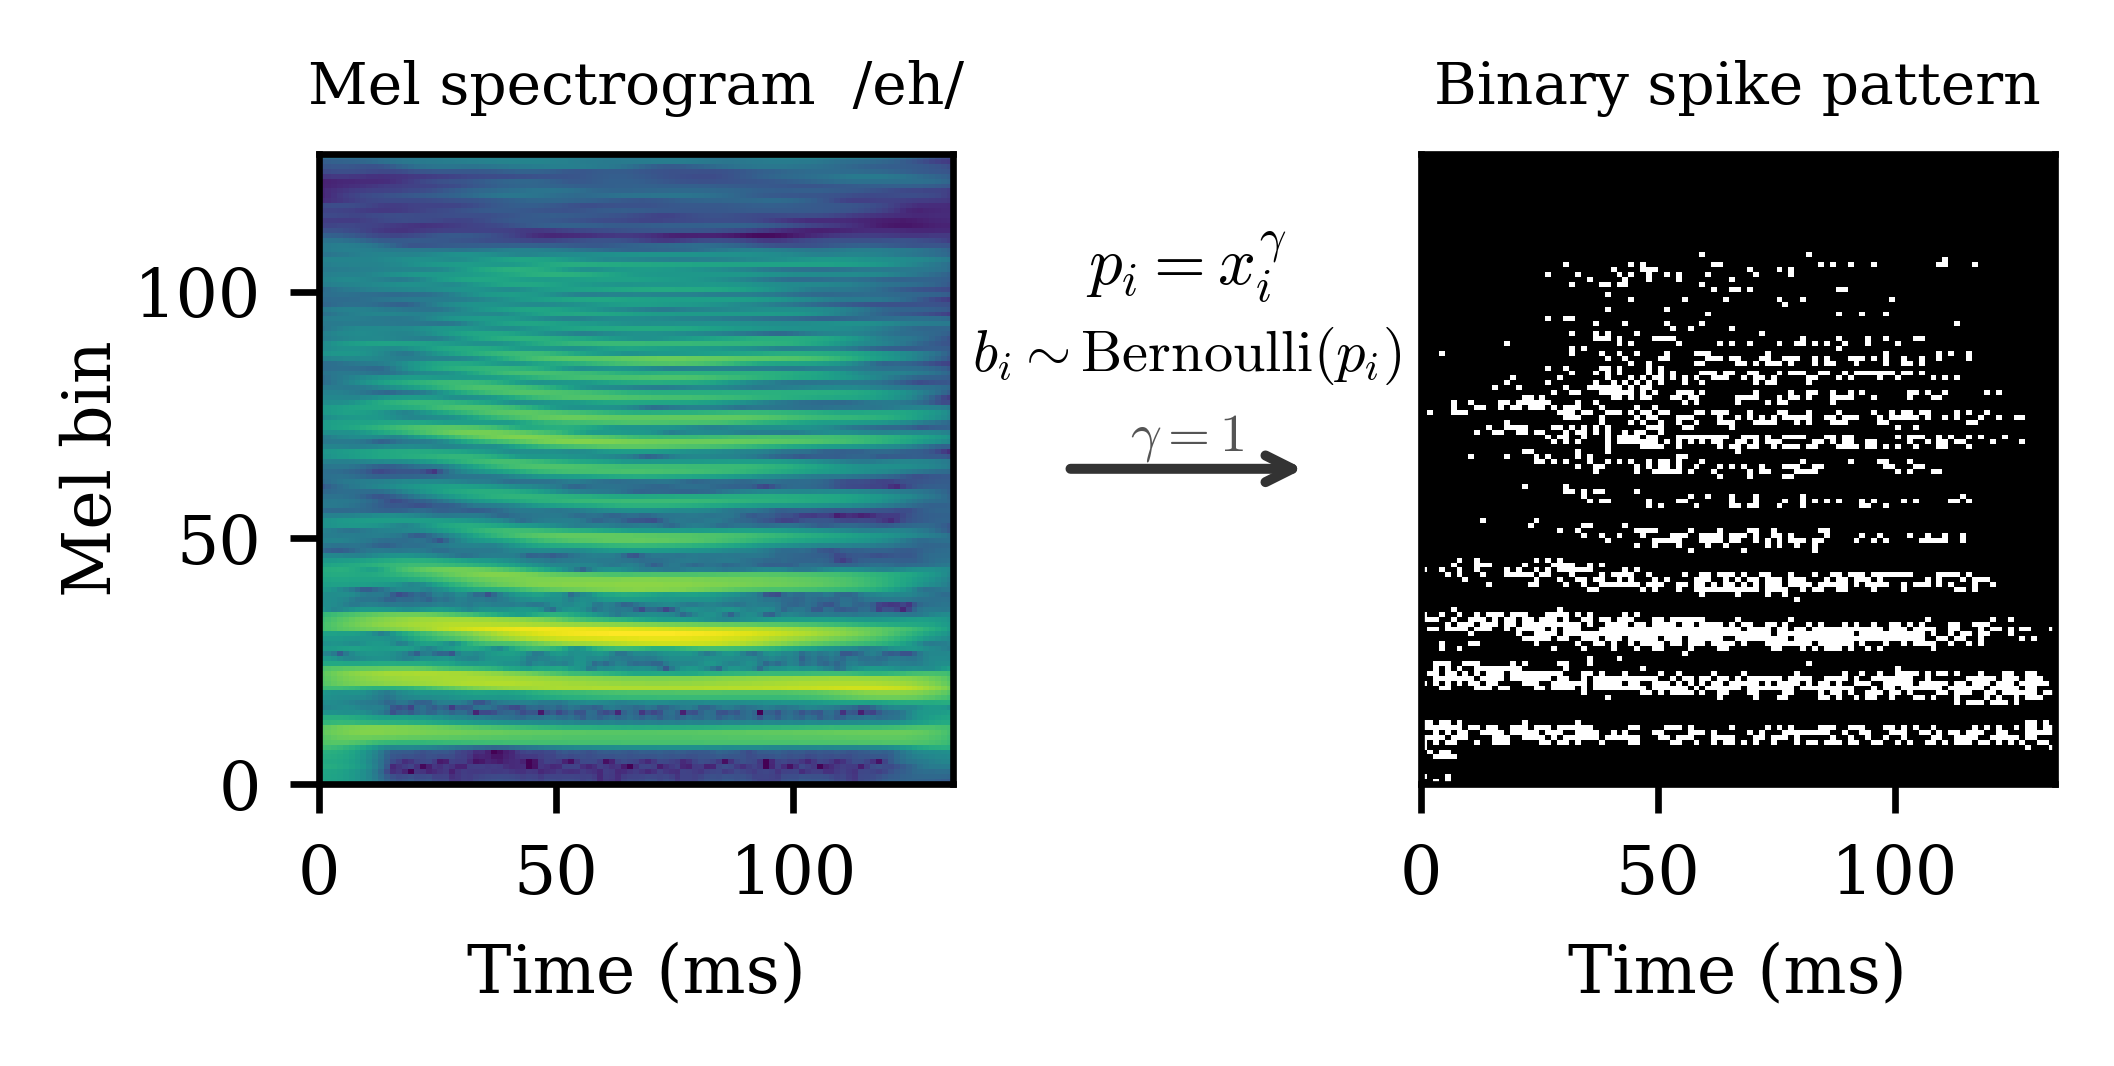
\includegraphics[width=\columnwidth]{figures/prob_binarisation.png}
    \caption{Probabilistic mel binarisation applied to a single phone segment (/eh/, 133\,ms). Left: continuous mel spectrogram normalised to $[0,1]$. Right: binary spike pattern obtained by treating each mel bin value as a Bernoulli firing probability. Brighter spectral regions produce denser activations.}
    \vspace{-10pt}
    \label{fig:prob_bin}
\end{figure}

\subsubsection{Population-Coded MFCC Encoding}
\label{sec:pop_mfcc}

While probabilistic mel encoding emphasises frame-to-frame change, recognition of quasi-stable acoustic categories (e.g., phones or words) benefits from features that are more invariant to pitch and speaker differences. For this purpose, we use Mel-Frequency Cepstral Coefficients (MFCCs) that are then mapped into sparse binary vectors via Gaussian population coding~\cite{quianquirogaPrinciplesNeuralCoding2013}.

As shown in Figure~\ref{fig:mfcc_pipeline}, each of the $M$ MFCC coefficients is represented by a population of $N_{\text{pop}}$ input neurons with Gaussian tuning curves. For coefficient $m$, we first compute the empirical range of its values over the training set and place the preferred values ${\mu_j}_{j=1}^{N{\text{pop}}}$ uniformly between the 1st and 99th percentiles, ensuring that the population tiles the range while being robust to outliers. Given a coefficient value $x$, the activation of neuron $j$ with preferred value $\mu_j$ and width $\sigma$ is: 
\begin{equation}
g_j(x) = \exp\left( -\frac{(x - \mu_j)^2}{2\sigma^2} \right)
\end{equation}

Stacking all $M$ coefficients and their $N_{\text{pop}}$-dimensional responses yields an $M \times N_{\text{pop}}$ continuous population code. We then binarise this code by thresholding each $g_j(x)$, producing a sparse binary input vector of dimensionality $n_{\text{input}} = M \times N_{\text{pop}}$. Neurons whose tuning curves are well-aligned with the current MFCC values become active, while others remain silent. This representation emphasises the overall spectral envelope shape rather than raw energy and yields structured, distributed binary patterns that are well-suited as inputs to AC areas in the classification pathway.


\begin{figure*}[t]
    \centering
    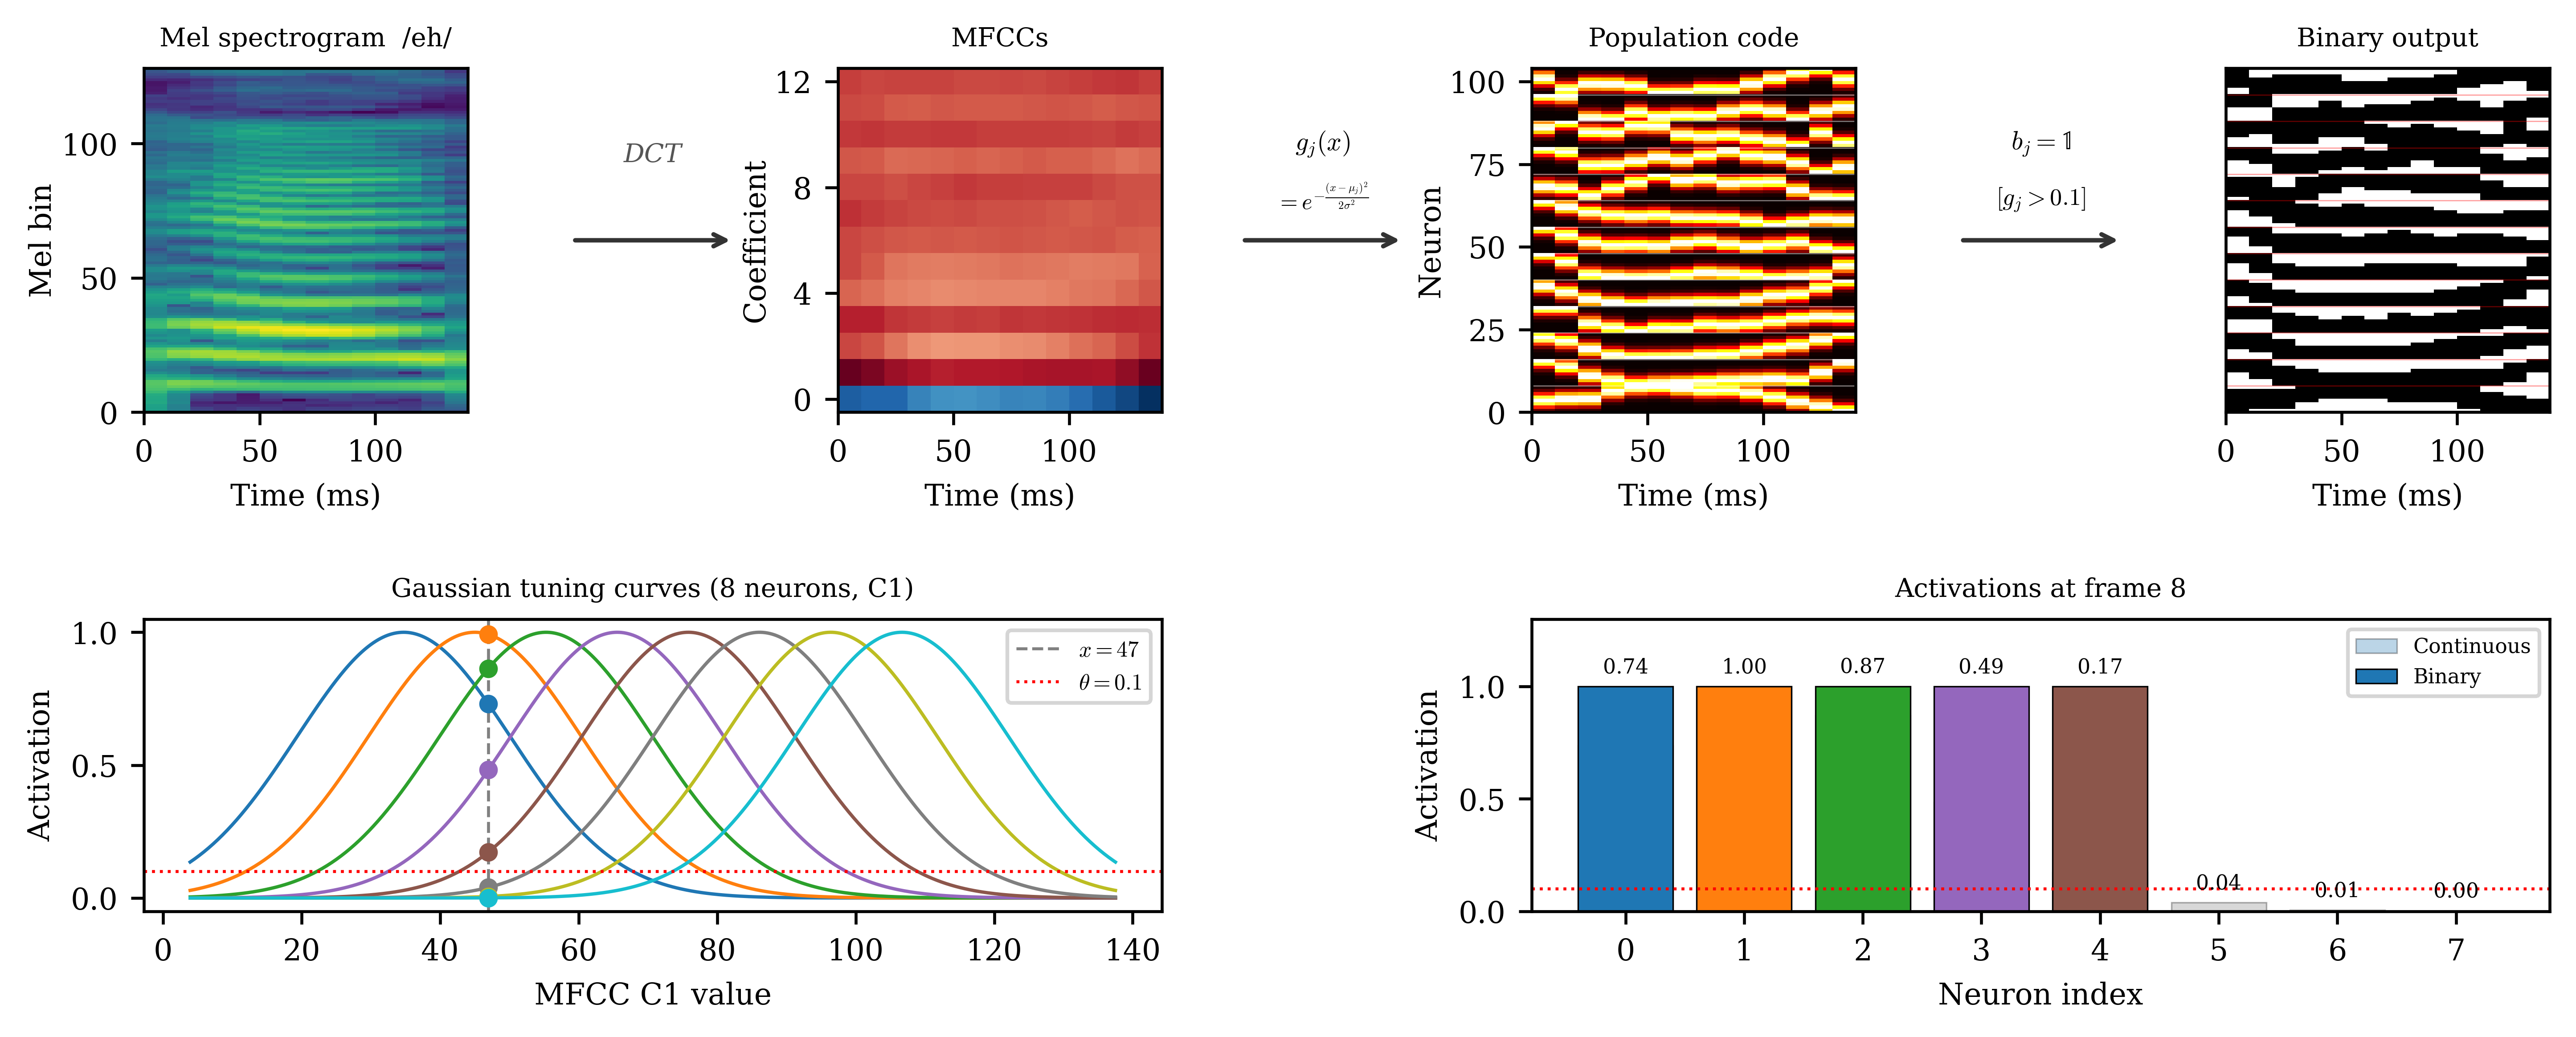
\includegraphics[width=\textwidth]{figures/mfcc_pipeline.png}
    \caption{Population-coded MFCC binarisation pipeline. Top row: mel spectrogram of a single phone (/eh/) is transformed into 13 MFCC coefficients, encoded by Gaussian tuning curves into a continuous population code, and thresholded to produce a sparse binary vector. Bottom row: detail of the Gaussian tuning curves for one coefficient (C1), showing how a single MFCC value activates overlapping neurons, and the resulting continuous and binary activations.}
    \vspace{-10pt}
    \label{fig:mfcc_pipeline}
\end{figure*}

Together, these two encodings provide a biologically plausible binary interface between continuous speech signals and discrete assembly dynamics, supporting sensitivity to fine-grained temporal changes and stable local state representations suitable for higher-level pattern formation respectively.

\subsection{Assembly for Segmentation and Classification}
Figure~\ref{fig:architecture} depicts how the two binary feature streams described in the previous section drive the dynamics of AC areas configured for our two target tasks: temporal segmentation and segment classification.
We employ two specialised area configurations. A \textit{refractory area} is an assembly area augmented with refractory suppression (Section~2.2) and operated without plasticity ($\beta{=}0$); its dynamics are driven entirely by feedforward input and refractory adaptation, making it sensitive to input changes. A \textit{per-class recurrent area} is a RecurrentArea dedicated to a single class and trained with plasticity ($\beta{>}0$); its learned recurrent weights encode class-specific temporal trajectories.
For temporal segmentation, binarised mel frames are processed by a hierarchy of refractory areas whose state changes expose phone- and word-level boundaries in continuous speech. For segment classification, population-coded MFCC sequences are presented to per-class recurrent areas whose learned assembly trajectories act as dynamical templates for phone and word categories. These constructions specify how binary inputs from the neural encoding are transformed into task-relevant assembly dynamics in our AC-based speech system.

\begin{figure}[t]
\centering

\tikzset{
  area/.style={draw, rounded corners=2pt, minimum height=0.50cm, minimum width=1.3cm,
               font=\scriptsize, inner sep=2pt, align=center, fill=blue!12, thick},
  output/.style={draw, rounded corners=2pt, minimum height=0.45cm, minimum width=1.1cm,
               font=\scriptsize, inner sep=2pt, align=center, fill=green!15},
  proc/.style={draw, rounded corners=2pt, minimum height=0.45cm, minimum width=0.5cm,
               font=\scriptsize, inner sep=2pt, align=center},
  input/.style={draw, rounded corners=2pt, minimum height=0.45cm, minimum width=1.1cm,
               font=\scriptsize, inner sep=2pt, align=center, fill=orange!12},
  score/.style={draw, rounded corners=2pt, minimum height=0.45cm, minimum width=0.45cm,
               font=\scriptsize, inner sep=2pt, align=center, fill=red!10},
  arr/.style={-{Stealth[length=3pt]}, thick},
}

\begin{tikzpicture}[x=1cm, y=1cm]

\node[font=\footnotesize\bfseries, anchor=west] at (-0.2, 1.15) {(a) Hierarchical Boundary Detection};

\node[input] (audio) at (0.4, 0.0) {Audio};

\node[input] (bin) at (2.1, 0.0) {Prob.\ mel\\[-1pt]binarisation};

\node[area] (l1) at (4.0, 0.0) {Level\,1\\[-1pt]\scriptsize Refract.\ Area};

\node[proc] (cs1) at (5.5, 0.0) {$c^{(t)}$};

\node[output] (phn) at (7.0, 0.0) {Phoneme\\[-1pt]boundaries};

\node[area] (l2) at (4.0, -1.0) {Level\,2\\[-1pt]\scriptsize Refract.\ Area};

\node[proc] (cs2) at (5.5, -1.0) {$c^{(t)}$};

\node[output] (wrd) at (7.0, -1.0) {Word\\[-1pt]boundaries};

\draw[arr] (audio) -- (bin);
\draw[arr] (bin) -- (l1);
\draw[arr] (l1) -- (cs1);
\draw[arr] (cs1) -- (phn);
\draw[arr] (l1.south) -- (l2.north) node[font=\tiny, right, xshift=1pt, midway] {$\mathbf{a}^{(t)}$};
\draw[arr] (l2) -- (cs2);
\draw[arr] (cs2) -- (wrd);

\node[font=\tiny\itshape, text=black!50] at (4.0, -1.55) {no learned weights ($\beta=0$)};

\end{tikzpicture}

\vspace{0.3cm}

\begin{tikzpicture}[x=1cm, y=1cm]

\node[font=\footnotesize\bfseries, anchor=west] at (-0.2, 1.95) {(b) Per-Class Phoneme Classification};

\node[input] (audio) at (0.4, 0.0) {Audio};

\node[input] (mfcc) at (2.1, 0.0) {Pop-coded\\[-1pt]MFCCs};

\coordinate (fanout) at (2.9, 0.0);

\node[area] (a1) at (4.2, 1.0) {RecurrentArea$_1$\\[-1pt]\scriptsize class: \textit{aa}};
\node[area] (a2) at (4.2, 0.0) {RecurrentArea$_2$\\[-1pt]\scriptsize class: \textit{ae}};
\node[font=\scriptsize] at (4.2, -0.55) {$\vdots$};
\node[area] (aC) at (4.2, -1.1) {RecurrentArea$_C$\\[-1pt]\scriptsize class: \textit{z}};

\node[score] (r1) at (5.9, 1.0) {$R_1$};
\node[score] (r2) at (5.9, 0.0) {$R_2$};
\node[score] (rC) at (5.9, -1.1) {$R_C$};

\node[output] (argmax) at (6.8, 0.0) {$\hat{c}$};

\draw[arr] (audio) -- (mfcc);
\draw[arr] (mfcc) -- (fanout);

\draw[arr] (fanout) |- (a1.west);
\draw[arr] (fanout) -- (a2.west);
\draw[arr] (fanout) |- (aC.west);

\draw[arr] (a1) -- (r1);
\draw[arr] (a2) -- (r2);
\draw[arr] (aC) -- (rC);

\draw[arr] (r1.east) -- ++(0.1,0) |- (argmax.north);
\draw[arr] (r2) -- (argmax);
\draw[arr] (rC.east) -- ++(0.1,0) |- (argmax.south);

\node[font=\tiny\itshape, text=black!50] at (4.2, -1.65) {Plasticity ($\beta>0$)};

\end{tikzpicture}

\caption{Architecture overview. \textbf{(a)}~Boundary detection: probabilistically binarised mel frames are processed by two cascaded refractory areas; the assembly change signal $c^{(t)}$ marks phoneme and word boundaries without any learned weights. \textbf{(b)}~Classification: population-coded MFCC frames are fed in parallel to $C$ independent per-class RecurrentAreas trained with Hebbian plasticity; the resonance score $R_c$ (Eq.~\ref{eq:resonance}) determines the predicted class $\hat{c} = \arg\max_c R_c$.}
\vspace{-15pt}
\label{fig:architecture}
\end{figure}


\subsubsection{Temporal Segmentation from Refractory Assembly Areas}
Temporal segmentation is formulated as an unsupervised boundary detection task, where the objective is to identify phone and word onset times in continuous speech.

We construct a hierarchy of two refractory areas that operate at different temporal scales and require no learned weights.
For a single area that consists of a population of neurons with recurrent connectivity and a $k$-cap operation, we obtain a sparse binary activity vector $\mathbf{a}^{(t)}$ with exactly $k$ active units. In addition, each neuron is subject to refractory suppression, meaning that recently active neurons are temporarily inhibited. This prevents the same set of neurons from persisting indefinitely and makes the area sensitive to changes in the input.

When synaptic plasticity is disabled ($\beta = 0$), the area functions purely as a dynamical system driven by three mechanisms: feedforward input, recurrent excitation among currently active neurons, and refractory adaptation. Given a sequence of sparse input frames $\{\mathbf{x}^{(t)}\}$, the area produces a trajectory of assemblies $\{\mathbf{a}^{(t)}\}$. If the input remains stable, the winning set of neurons tends to overlap strongly across consecutive frames. When the input distribution changes sufficiently, the competitive dynamics select a different set of $k$ neurons, resulting in a rapid reconfiguration of the assembly.

\noindent\textbf{Phone-scale segmentation (Level 1).}
The Level~1 area receives frame-level binary inputs obtained from probabilistic mel binarisation. Through $k$-cap competition, even moderate shifts in input statistics can alter which neurons win the competition. Refractory suppression further amplifies this sensitivity by discouraging persistence of the previous assembly. As a result, phone transitions produce noticeable reconfigurations in $\mathbf{a}^{(t)}$.

\noindent\textbf{Word-scale segmentation (Level 2).}
The Level~2 area operates on the activity of Level~1 rather than directly on acoustic input. It receives $\mathbf{a}^{(t)}$ as its input stream and applies the same competitive and refractory dynamics, but effectively integrates information over a longer timescale. Because words consist of structured sequences of phone-level assemblies, Level~2 becomes sensitive to larger-scale shifts in the pattern of Level~1 activity. When a word boundary occurs, the distribution of Level~1 assemblies changes more substantially, leading to a stronger reconfiguration at Level~2.

\noindent\textbf{Boundary signal.}
To quantify assembly reconfiguration at either level, we define the change measure:
\begin{equation}
c^{(t)} = 1 - \frac{\mathbf{a}^{(t)} \cdot \mathbf{a}^{(t-1)}}{k}
\label{eq:change}
\end{equation}
Since the dot product counts the number of shared active neurons between consecutive time steps, $c^{(t)}$ measures the fraction of neurons that have changed. Values near zero indicate stable assemblies, while large values indicate abrupt reorganisation. Peaks in $c^{(t)}$ therefore serve as intrinsic boundary indicators.
\begin{figure}[t]
    \centering
    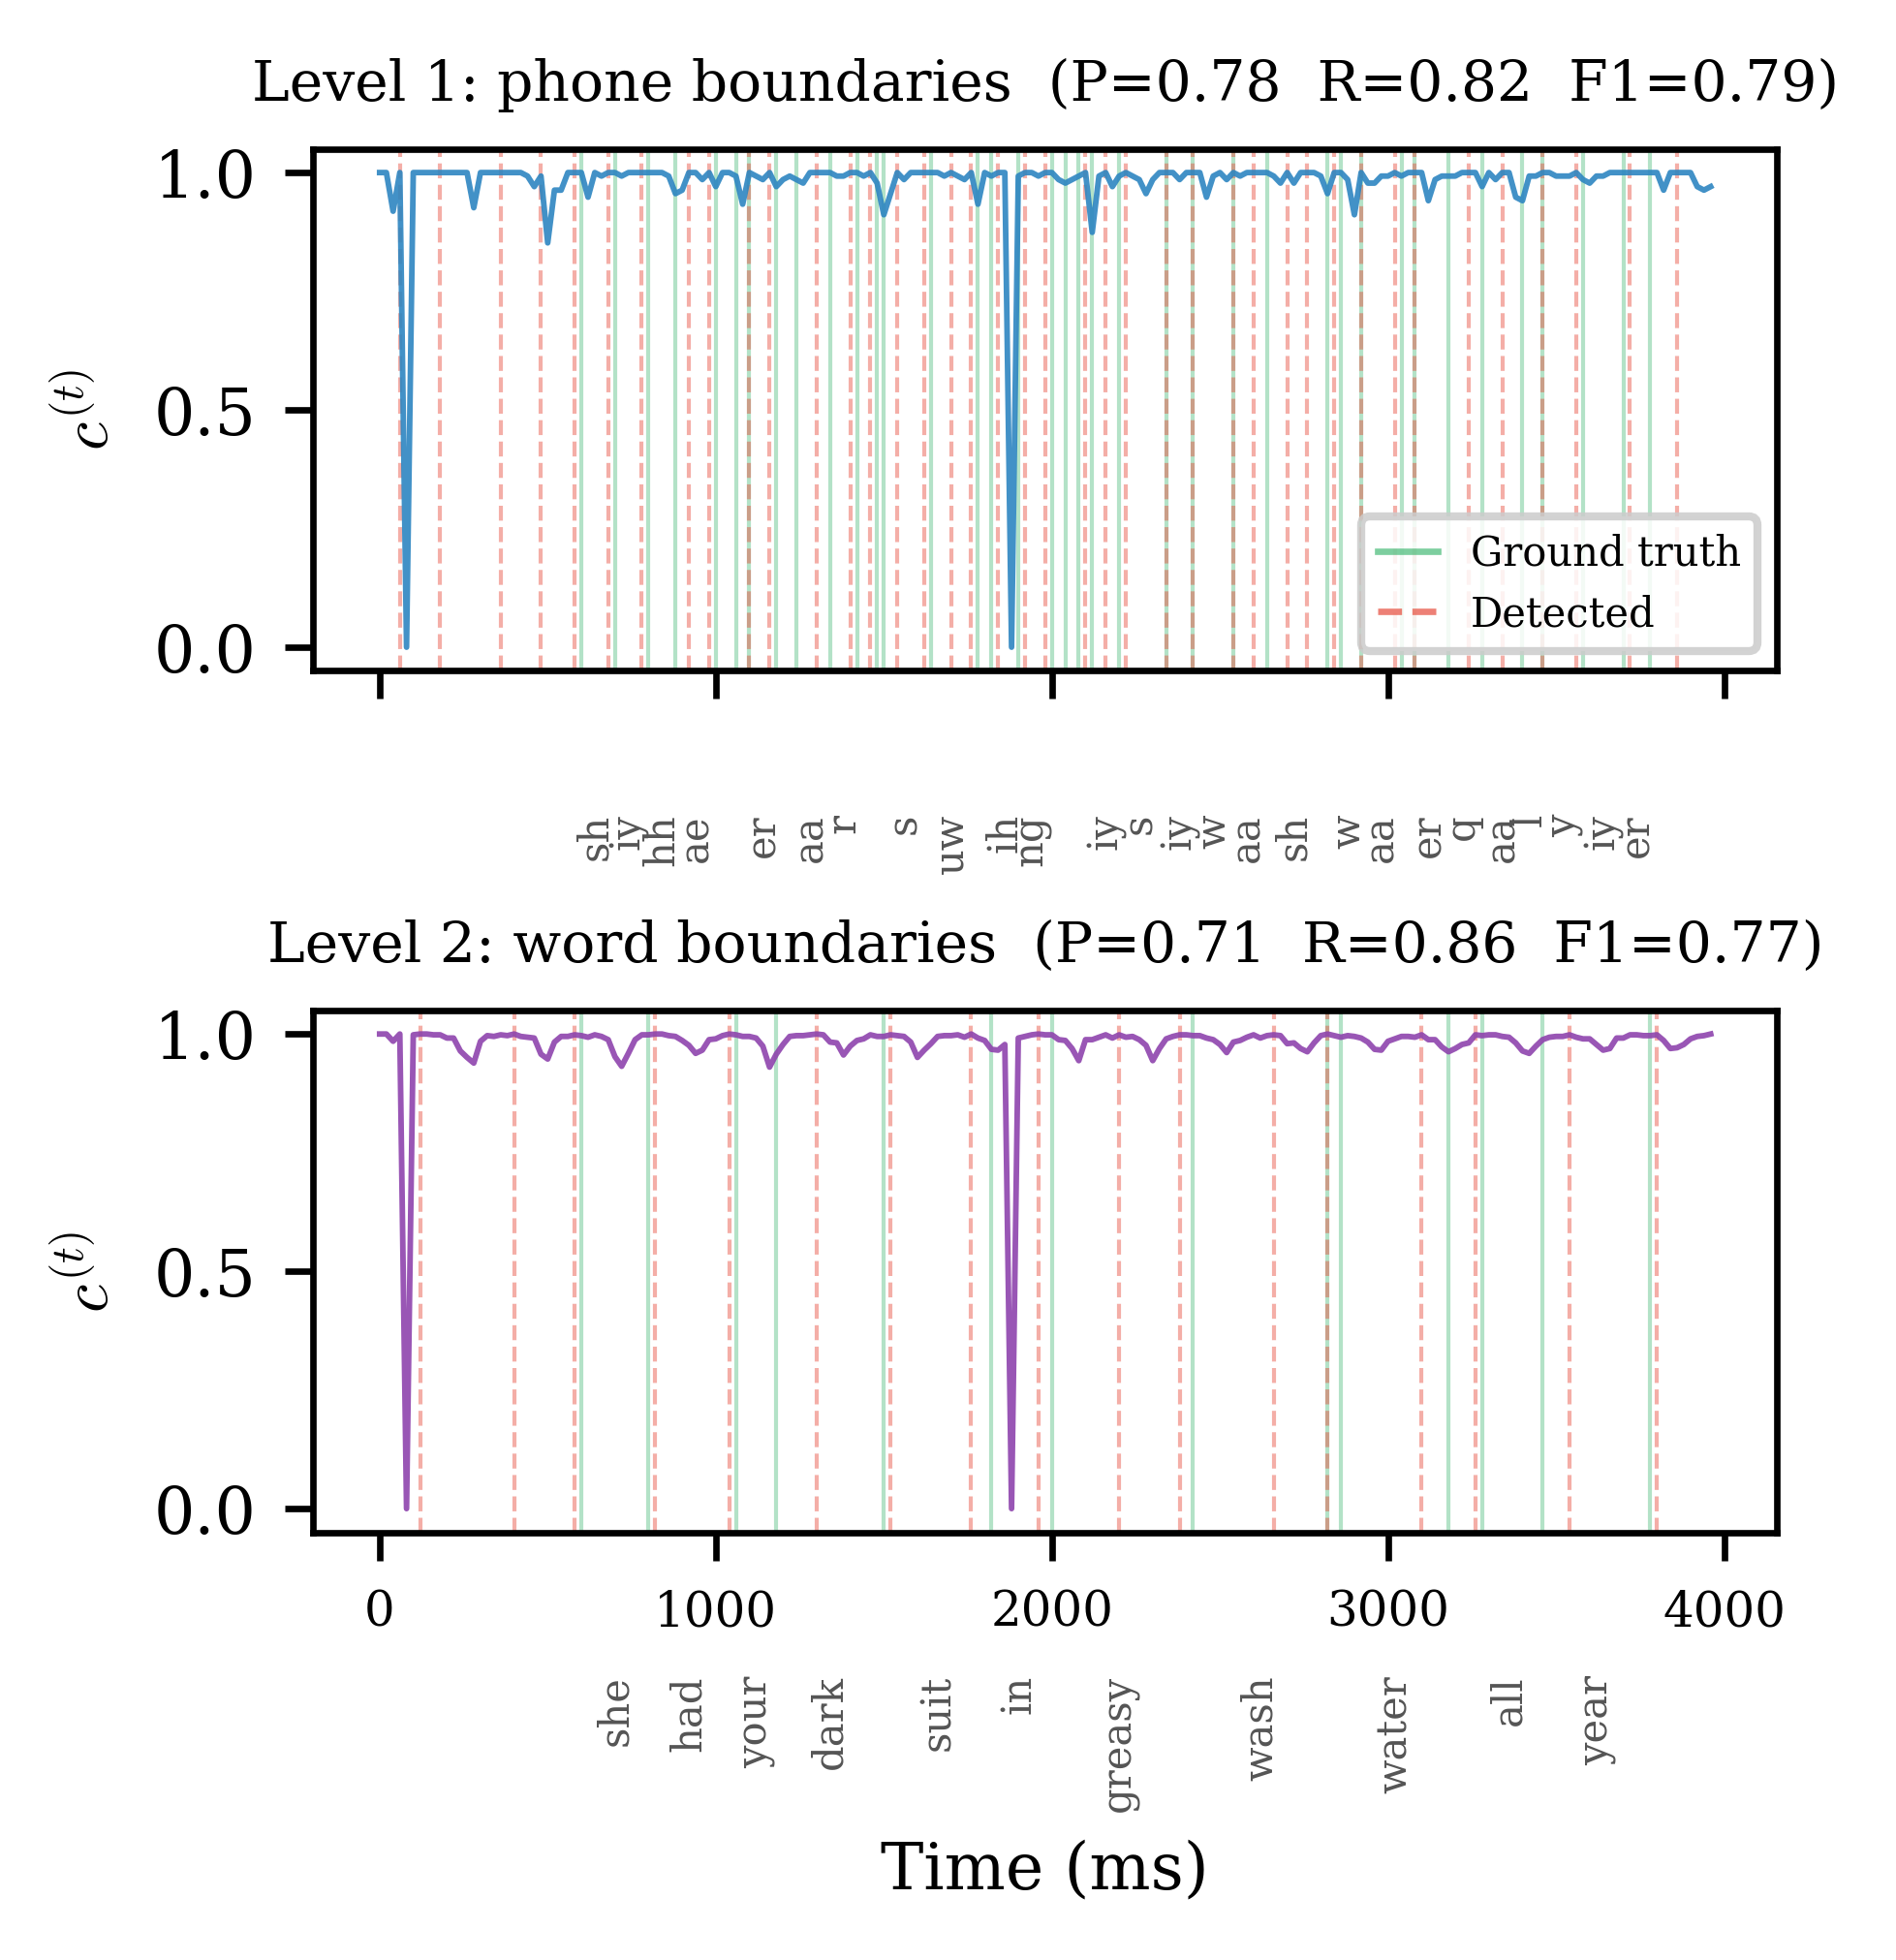
\includegraphics[width=0.9\columnwidth]{figures/boundary_signal.png}
    \caption{Assembly change signal $c^{(t)}$ (Eq.~\ref{eq:change}) for a single TIMIT utterance. \textbf{Top:} Level~1 (phone boundaries). \textbf{Bottom:} Level~2 (word boundaries). Green vertical lines mark ground-truth boundaries; red dashed lines mark detected peaks. Phone/word labels are shown below each axis.}
    \vspace{-10pt}
    \label{fig:boundary_signal}
\end{figure}


Importantly, both phone- and word-level segmentation emerge without supervised boundary labels or gradient-based optimisation. They arise directly from sparse competition and refractory adaptation operating at different hierarchical levels.

\subsubsection{Segment Classification from Trajectory Scoring}
While temporal segmentation operates in a non-plastic regime and detects boundaries through assembly reconfiguration, segment classification uses the same competitive assembly dynamics in a plastic regime to learn class-specific temporal structure.

We formulate phone classification as a supervised segment classification task using a bank of class-specific recurrent assembly areas. Concretely, we instantiate one \emph{RecurrentArea} per phone class, yielding $C$ independent dynamical systems. Each area learns the characteristic spectro-temporal trajectory of a single phone class.
Acoustic input is represented using population-coded mel-frequency cepstrum coefficients (MFCCs)~\cite{Davis80-COP} (Section~\ref{sec:pop_mfcc}), producing a sparse high-dimensional binary vector $\mathbf{x}^{(t)}$ at each frame.

\noindent\textbf{Recurrent assembly dynamics.}
Each RecurrentArea consists of a neuronal population governed by the same $k$-cap competition principle used in boundary detection. At each time step, neurons receive:
(i) feedforward input from the current acoustic frame via weights $\mathbf{W}^{\mathrm{ff}}$, and
(ii) recurrent input from the previous assembly via weights $\mathbf{W}^{\mathrm{rec}}$.

The total pre-competition input to area $c$ at time $t$ is
\begin{equation}
\mathbf{u}_c^{(t)} =
\mathbf{W}_c^{\mathrm{ff}} \mathbf{x}^{(t)}
+
\mathbf{W}_c^{\mathrm{rec}} \mathbf{a}_c^{(t-1)},
\end{equation}
As before, a $k$-cap rule selects the $k$ neurons with largest total input to form the active assembly $\mathbf{a}_c^{(t)}$. Thus, classification relies on the same sparse competitive mechanism as segmentation; the difference lies in the presence of synaptic plasticity.

\noindent\textbf{Plastic learning of phone dynamics.}
When plasticity is enabled, area $c$ is exposed only to contiguous segments belonging to phone class $c$. Segments are presented in temporal order, allowing the area to learn not just static spectral patterns but their characteristic evolution across time.

Between segments, activations are reset so that each segment begins from a neutral state. This mirrors the ``cold start'' assumption in segmentation and prevents cross-segment interference.

Through repeated exposure, feedforward weights strengthen connections from frequently co-occurring input features, while recurrent weights reinforce transitions between successive assemblies. Consequently, each area internalises a dynamical signature of its phone class: feedforward structure encodes typical spectral evidence, and recurrent structure encodes the typical progression of that evidence.

\noindent\textbf{Resonance-based trajectory scoring}
\label{sec:traj_scoring}
At test time, plasticity is disabled, and a candidate segment is sequentially presented to all $C$ areas. Each area generates an internal assembly trajectory driven by its learned weights.

If the input trajectory aligns with the learned class-specific dynamics of area $c$, feedforward and recurrent inputs reinforce one another over time. This produces consistently strong pre-competition activation values. If the trajectory is inconsistent, recurrent support is weaker and activation remains lower.
\begin{figure*}[t]
\centering
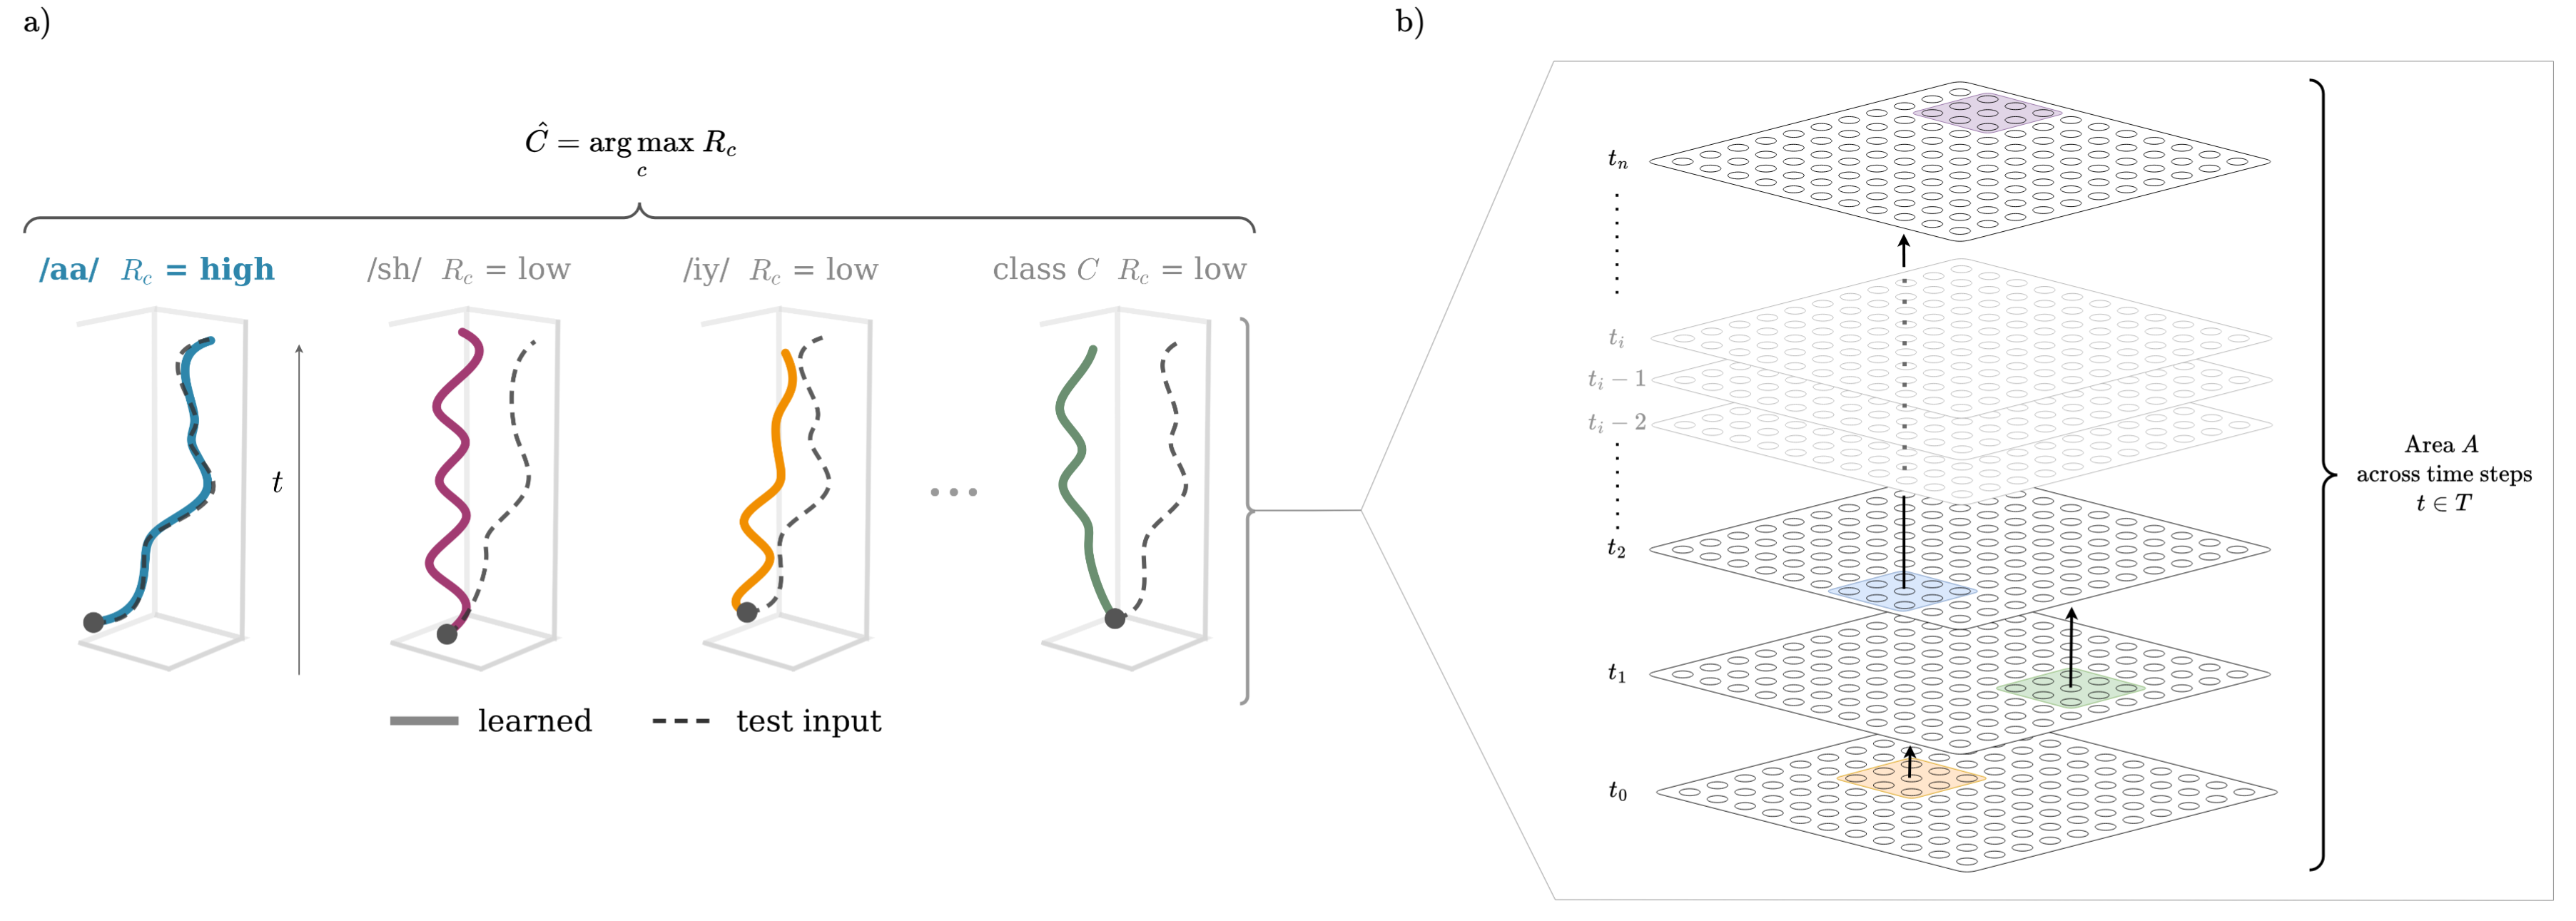
\includegraphics[width=0.9\textwidth]{figures/trajectories_with_detail_horizontal.png}
\caption{Trajectory-based resonance scoring. Each of $C$ per-class RecurrentAreas (a) has learned a characteristic trajectory through assembly space (solid, coloured). The same test input (dashed) is presented to all areas in parallel. The inset (b) shows the frame-by-frame operation: feedforward drive from the current input combines with recurrent drive from the previous assembly, and the top-$k$ neurons fire. The predicted class is the label of the area with the learned trajectory that most closely matches the input, as measured by the resonance score $R_c$.}
\vspace{-15pt}
\label{fig:trajectory}
\end{figure*}


We quantify this alignment using a resonance score:
\begin{equation}\label{eq:resonance}
    R_c = \frac{1}{T'}
    \sum_{t}
    \sum_{i=1}^{k}
    \mathrm{topk}_i\bigl(\mathbf{u}_c^{(t)}\bigr),
\end{equation}
where $T'$ is the number of frames in the segment and $\mathrm{topk}_i(\mathbf{u})$ denotes the $i$-th largest element of $\mathbf{u}$, so the inner sum computes the total pre-competition activation of the $k$ winning neurons. This score measures the cumulative amplification of the input trajectory by the area's learned feedforward and recurrent structure. 
The predicted label is
\begin{equation}
    \hat{c} = \arg\max_c R_c.
\end{equation}

Both segmentation and classification arise from the same underlying assembly dynamics. In segmentation, abrupt changes in assembly configuration (quantified by Eq.~\ref{eq:change}) signal temporal boundaries in a non-plastic regime. In classification, plasticity shapes recurrent structure so that entire trajectories resonate within a class-specific dynamical system. 

Thus, boundaries are detected through transient instability of assemblies, whereas classes are identified through sustained dynamical alignment. In both cases, computation emerges from sparse competition and temporal recurrence rather than gradient-based sequence modeling (Figure~\ref{fig:trajectory}).
